% generated by scripts/pkl_to_latex.py
% source PKL : uscan_v1_L6_Ne5_t1_mode-uniform_nmin2_solver-gcg_full_restarts10_iter300_kmax4_tol1em09_U1to20_N21-cc2ba367e4e0.pkl
% scan type  : uscan
% state      : gs
% requires   : \usepackage{pgfplots} \pgfplotsset{compat=1.18}
% colours match the matplotlib PDF (tab10 cycle)
\definecolor{gmeC0}{HTML}{1F77B4}
\definecolor{gmeC1}{HTML}{FF7F0E}
\definecolor{gmeC2}{HTML}{2CA02C}
\definecolor{gmeC3}{HTML}{D62728}
\definecolor{gmeC4}{HTML}{9467BD}
\definecolor{gmeC5}{HTML}{8C564B}
\definecolor{gmeC6}{HTML}{E377C2}
\definecolor{gmeC7}{HTML}{17BECF}

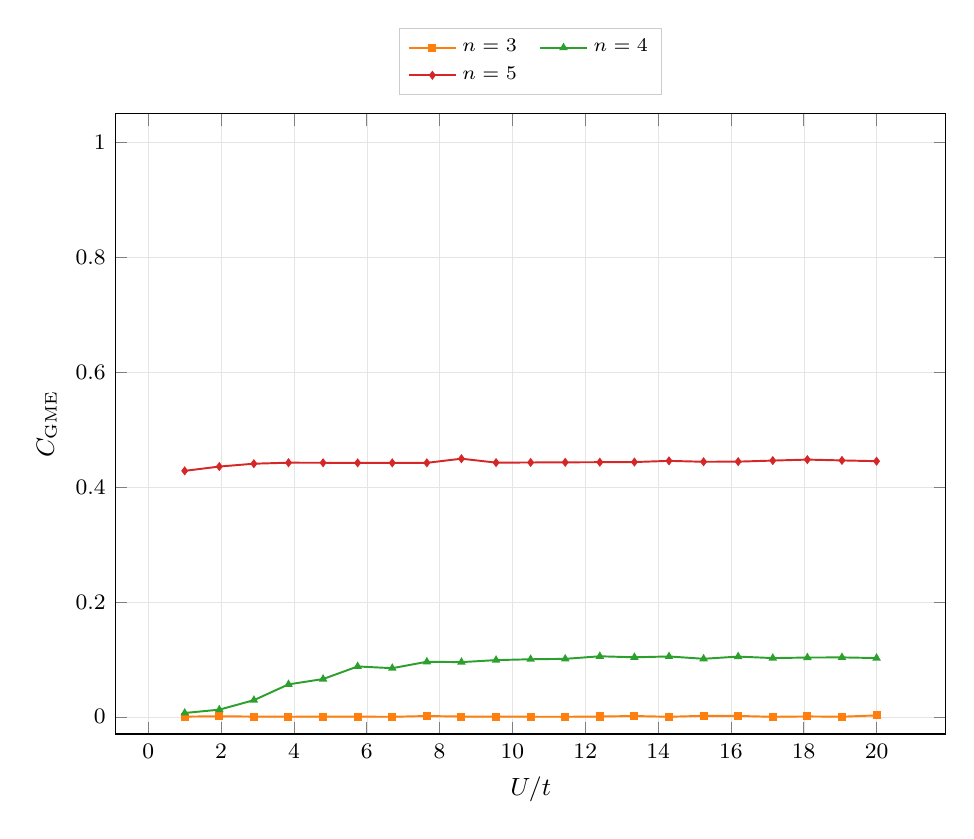
\begin{tikzpicture}
  \begin{axis}[
    width=\columnwidth,
    height=0.78\columnwidth,
    xlabel={$U/t$},
    ylabel={$C_{\mathrm{GME}}$},
    grid=both,
    grid style={line width=.1pt, draw=gray!20},
    tick label style={font=\footnotesize\rmfamily, /pgf/number format/fixed},
    label style={font=\small\rmfamily},
    scaled ticks=false,
    legend style={font=\scriptsize\rmfamily, draw=gray!40, at={(0.5,1.03)}, anchor=south, /tikz/every even column/.append style={column sep=6pt}},
    legend cell align={left},
    legend columns=2,
    ymin=-0.03,
    ymax=1.05,
  ]
    \addplot[color=gmeC1, mark=square*, mark size=1.1pt, line width=0.7pt] coordinates {
        (1,0.000363) (1.95,0.000951) (2.9,0.000398) (3.85,0.000117)
        (4.8,0.000314) (5.75,0.000278) (6.7,0.000051) (7.65,0.00138)
        (8.6,0.000478) (9.55,0.000238) (10.5,0.000148) (11.45,0.000033)
        (12.4,0.00054) (13.35,0.001387) (14.3,0.000094) (15.25,0.001697)
        (16.2,0.001496) (17.15,0.000023) (18.1,0.000676) (19.05,0.000191)
        (20,0.002451)
    };
    \addlegendentry{$n=3$}
    \addplot[color=gmeC2, mark=triangle*, mark size=1.1pt, line width=0.7pt] coordinates {
        (1,0.006699) (1.95,0.012409) (2.9,0.029007) (3.85,0.056459)
        (4.8,0.06579) (5.75,0.087699) (6.7,0.084661) (7.65,0.095855)
        (8.6,0.095222) (9.55,0.098734) (10.5,0.100225) (11.45,0.100916)
        (12.4,0.105397) (13.35,0.103648) (14.3,0.105096) (15.25,0.101049)
        (16.2,0.104879) (17.15,0.102272) (18.1,0.103196) (19.05,0.103456)
        (20,0.102323)
    };
    \addlegendentry{$n=4$}
    \addplot[color=gmeC3, mark=diamond*, mark size=1.1pt, line width=0.7pt] coordinates {
        (1,0.428306) (1.95,0.435799) (2.9,0.440751) (3.85,0.442523)
        (4.8,0.442383) (5.75,0.442245) (6.7,0.44221) (7.65,0.442281)
        (8.6,0.449485) (9.55,0.44264) (10.5,0.442879) (11.45,0.443134)
        (12.4,0.443392) (13.35,0.443648) (14.3,0.445688) (15.25,0.444136)
        (16.2,0.444364) (17.15,0.446197) (18.1,0.447919) (19.05,0.446488)
        (20,0.445159)
    };
    \addlegendentry{$n=5$}
  \end{axis}
\end{tikzpicture}
